% EN49 c06 | 原书 原书 p.58–64（PDF 69–75） | 第 4 章 §4.1
% 骨架文件：标题行已设定，正文由译者填写。每页起首用 % ===== 原书 p.N ===== 注释标记。
\section{超曲面的 Kn{\"o}rrer 周期性}

\subsection{AAK 等价}

% ===== 原书 p.58 =====
我们先证明超曲面情形的光滑 Kn{\"o}rrer 周期性，即定理 \ref{thm:aak-equiv}（Abouzaid--Auroux--Katzarkov 等价）：

\begin{thmstar}
设 $X$ 是光滑仿射簇，带嵌入 $X\to\C^N$，该嵌入在 $X$ 上诱导 Stein 结构；设
$f\colon X\to\C$ 是 $\C^N$ 上多项式函数的限制。若 $f$ 只有一个临界纤维
$f^{-1}(0)$，则对充分小的 $t\neq0$，存在 $A_\infty$ 范畴的拟等价
\[
T\colon\cW(f^{-1}(t))\to\cW(X\times\C,z(f-t)),
\]
\end{thmstar}

\transnote{易错预警：原书在第 4 章开头把引言中的定理 \ref{thm:aak-equiv} 原样重述，并沿用原编号。
译本编号全部自动生成，若另立有编号的定理环境，同一结论会得到「4.1.1」的新号，还会把
紧随其后的那条定义挤成下一号。故此处用无编号的 thmstar 环境，编号一律引
定理 \ref{thm:aak-equiv}。后文重述定理 \ref{thm:relative}、\ref{thm:knorrer} 同此处理。}

% ===== 原书 p.59 =====
该函子由在奇异轨迹 $f^{-1}(t)$ 中的可容拉格朗日子流形上取顶针给出。

首先，我们要描述证明中将在 $(X\times\C,z(f-t))$ 上使用的 Liouville 结构与近复结构
（almost-complex structure）。
以下记 $F_t=z(f-t)$。这里想提醒读者注意注 \ref{rem:6} 中的约定，即如何为
Landau--Ginzburg 模型的单个临界值构造局部 Liouville 扇形。

\transnote{含糊点拨：原书此处只写「Remark 6」，未带节号，页图上该编号也不是红色链接；
它应指第 2 章里按独立序列编号的第 6 条注，但底本没有给出更精确的定位。译本按第 2 章的
注记编号引作「注 6」，正文照译，不补猜测。}

首先，由命题 \ref{prop:2-2-6}，因 $t\neq0$ 时 $f^{-1}(t)$ 光滑，我们可以把
$V=f^{-1}(B_\delta(t))$ 光滑地等同于 $f^{-1}(t)\times\C$，其中 $B_\delta(t)$ 是
$t\in\C$ 附近的小球。于是在这个开集 $V\times\C$ 上，映射
$F_t\colon X\times\C\to\C$ 由局部 Morse--Bott 模型
$f^{-1}(t)\times\C^2\to\C$ 显式给出：$(x,y)\mapsto xy$，其中 $x,y$ 是 $\C^2$ 中的坐标。

\transnote{背景直觉：这个局部模型把 $F_t$ 在光滑纤维邻域内化归为 $\C^2$ 上的结点模型
$x\mapsto xy$。$x$ 沿纤维方向、$y$ 沿底空间方向，正是后文「在逐纤维的无穷远处柱状」
这一说法的来源。}

由命题 \ref{prop:2-2-6}，在 $f\colon X\to\C$ 光滑平凡的开集 $U$ 上，存在 Liouville
形变 $\lambda_t$，把 Liouville 结构变为 $f^{-1}(U)\cong f^{-1}(t)\times U$ 上的乘积型
Liouville 结构。可以让这个形变在更大的开集之外保持常值；由于该形变保持纤维，它是一次
简单 Liouville 同伦（定义 \ref{def:2-1-5}）。我们先把这一构造用于 $U=B_\delta(t)$，
即光滑纤维 $f^{-1}(t)$ 的一个小邻域，其中不含 $f$ 的临界点。再过渡到乘积
$f^{-1}(B_\delta(t))\times\C$，$\C$ 上取标准 Liouville 结构；所得形变仍为简单形变，
它给出 $F_t$ 在 $-\infty$ 上方纤维的一条同痕。由引理 \ref{lem:2-1-6}，该形变不改变
$(X\times\C,F_t)$ 的 wrapped Fukaya 范畴，因此在证明中可以放心改用这个改动后的
Liouville 结构。注意，该形变不改变 $f^{-1}(t)$ 上诱导的 Liouville 结构。

\transnote{含糊点拨：「简单 Liouville 同伦」指形变过程保持纤维、且只在紧集内改动；
引理 \ref{lem:2-1-6} 保证这种改动不改变 wrapped Fukaya 范畴。作者借此把一般 Liouville
结构换成便于计算的乘积型结构，而不损失范畴层面的信息。}

我们把这一论证再用一次，这次用于纤维丛 $F_t\colon X\times\C\to\C$：在子集
$\{\operatorname{Re}(z)>0\}\cup\{\operatorname{Im}(z)>0\}$ 上（当然要与 §2 中的小圆盘
取交），可以再次把 Liouville 结构形变为乘积型，其中底空间取径向 Liouville 结构。

\transnote{背景直觉：选这个扇形区域是为了让 Reeb 流在底空间里表现为旋转。于是
「逆时针」「顺时针」都可按底空间的角坐标比较，后文对 马斯洛夫指数的计算依赖这一点。}

% ===== 原书 p.60 =====
注意，该形变保持光滑纤维 $X\setminus f^{-1}(t)$ 上的 Liouville 结构不变。我们同样可以在
论证中改用 $X\times\C$ 上的这个 Liouville 结构。

现在可以让等同 $F_t\colon f^{-1}(B_\delta(t))\times\C\to\C$ 与映射
$f^{-1}(t)\times\C^2\to\C$、$(x,y)\mapsto xy$ 相容于近复结构。在 $f^{-1}(t)$ 与 $X$
上取柱状近复结构，在 $\C$ 上取标准复结构。我们先修改 $X$ 上的复结构，使它在
$F_t^{-1}(D)\times\C$ 内（$D\subseteq\C$ 是 $0$ 附近的小开圆盘）与
$f^{-1}(t)\times\C$ 上的乘积近复结构一致，再在这个开子集之外与通常的近复结构作插值。
由于 Liouville 结构在 $f^{-1}(t)$ 附近是乘积型，所得的 $X\times\C$ 上近复结构显然也可
取为柱状。对 $\C$ 上任何（柱状）近复结构都可以重复这一构造。

\transnote{含糊点拨：页图此处印作 $F_t^{-1}(D)\times\C$，但 $F_t^{-1}(D)$ 本身已是
$X\times\C$ 的子集，再乘 $\C$ 在类型上说不通；按上下文，作者应是想说「在
$F_t^{-1}(D)$ 这个开集内」。译文照录原式，不改动，并把这一处列入报告疑点。}

\begin{proof}[定理 \ref{thm:aak-equiv} 的证明]
首先选取 $f^{-1}(t)$ 内一族柱状正合 $\Spin$ 拉格朗日子流形 $L_i$，$i\in I$，它们代表
$f^{-1}(t)$ 上诱导 Stein 结构的余核（cocore）。对每个拉格朗日子流形，考虑其上的顶针
$T_i$：从 $L_i\subseteq f^{-1}(t)$ 出发，在 $X\times\C$ 内沿 $\operatorname{Re}(F_t)$
的归一化梯度流扫出。由于每个 $L_i$ 正合，这些 $T_i$ 是 $X\times\C$ 的正合拉格朗日子流形；
从 $T_i$ 到 $L_i$ 的形变收缩为它们配上 $\Spin$ 结构。我们断言，这些 $T_i$ 也可以取成
柱状的。

\transnote{易错预警：术语 cocore 译作「余核」，指手柄的稳定流形，与代数学的「余核」
（cokernel）无关；首次出现括注英文，后文径称余核。$\Spin$ 结构是拉格朗日子流形上用于给
圆盘模空间定向的数据，译本保留符号 $\Spin$，不音译。}

首先，存在充分小的 $\varepsilon>0$，使得在 $B_\varepsilon(0)$ 上方，顶针 $T_i$ 完全落在
Morse--Bott 局部模型 $f^{-1}(B_\delta(t))\times\C$ 内；理由是 $f^{-1}(B_\delta(t))$ 上的
正合辛结构是乘积。

% ===== 原书 p.61 =====
在局部 Morse--Bott 模型中可以直接验证：在 $F_t^{-1}(0)$ 附近，$T_i$ 在逐纤维的无穷远处
是柱状的——它们由 $L_i$ 与 $\C^2$ 内标准 Lefschetz 顶针的乘积给出。现在还需在底空间的
无穷远处核对。在邻域 $B_\varepsilon(0)$ 之外（所有拉格朗日子流形的交点都在该邻域内），
可以改用 Liouville 向量场流动，而不作平行移动，使所得拉格朗日子流形在 $\infty$ 处柱状。

现在，对每个 $T_i$ 取共尾序列（cofinal sequence）$T_i^{(t)}$：这里用
[GPS20b, Lemma 3.29] 中构造的完备 Reeb 向量场的时间 $t$ 流，并取一般位置，以保证有限
全序集上相交的横截性（见 [GPS20b, Definition 3.34]）。由于 Liouville 结构在
$\{\operatorname{Re}(z)>0\}$ 上是乘积型，任何 Reeb 流都由底空间中的旋转给出；于是可以取
紧支哈密顿同痕，使 $T_i^{(t)}$ 位于 $B_\varepsilon(0)$ 内的一条射线上方。取 $L_i^{(t)}$
为 $T_i^{(t)}$ 与临界轨迹的交；由 [GPS20b, Lemma 3.29]，$L_i^{(t)}$ 也构成共尾序列，
因为量
\[
\int_0^\infty \min_{\partial_\infty L_t}\alpha(\partial_\infty\partial_t L_t)\,dt
\]
在限制到更小的集合时只会增大。为定义 $\cW(X\times\C,F_t)$，选取一族带共尾序列的
拉格朗日子流形，并把 $T_i^{(t)}$ 作为子族包含在内。

\transnote{易错预警：$T_i^{(t)}$ 的上标 $t$ 是 Reeb 流的时间参数，不是纤维参数 $t$；
同一段里两种 $t$ 混用，对照页图时须分清。积分式中的 $L_t$ 是随流时间变化的拉格朗日
子流形，$\partial_\infty$ 指其无穷远处的边界。}

现在考虑由 $f^{-1}(t)$ 内的 $L_i^{(j)}$ 给出的有向 Fukaya 范畴 $\cO$，以及由
$(X\times\C,F_t)$ 内的 $T_i^{(t)}$ 给出的有向 Fukaya 范畴 $\cA$，如
[GPS20b, Definition 3.35]。当 $j>j'$ 时，$\cA(T_i^{(j)},T_{i'}^{(j')})$ 由 Floer 复形
$CF(T_i^{(j)},T_{i'}^{(j')})$ 给出：在底空间中，$T_i^{(j)}$ 位于从
$T_{i'}^{(j')}$ 逆时针转过的一条径向射线上方，因而二者只在纤维 $F_t^{-1}(0)$ 中相交，
交点正是横截交点 $L_i^{(j)}\cap L_{i'}^{(j')}$。因此
\[
\cA(T_i^{(j)},T_{i'}^{(j')})=\cO(L_i^{(j)},L_{i'}^{(j')}).
\]
马斯洛夫指数在乘积下的可加性，以及 $T_i^{(j)}$ 位于 $T_{i'}^{(j')}$ 严格逆时针方向的
径向射线上方这一事实，说明这是分次向量空间的同构。当 $j\le j'$ 时，态射空间显然相同。
接下来要匹配两个有向范畴上的 $A_\infty$ 运算。

% ===== 原书 p.62 =====
给定一族顶针 $T_i^{(j_n)}$，$n=0,\dots,k$，其中 $j_0>\cdots>j_k$；选取适当的
（依赖于定义域与共形结构（conformal structure）的）$f^{-1}(t)$ 上的柱状近复结构 $J$，使定义 $L_i^{(j_n)}$ 的
运算 $\mu^k$ 所用的模空间正则（如 [GPS20b, p.41]），再按上述方式把它们延拓为
$X\times\C$ 上的柱状近复结构。相对于这样的近复结构，映射
$F_t\colon X\times\C\to\C$ 在包含 $L_i^{(j_n)}$（从而包含 $T_i^{(j_n)}$）所有交点的
一个开集上为 $J$-全纯。因此，对定义 $T_i^{(j_n)}$ 的运算 $\mu^k$ 的任一全纯圆盘，它在
$F_t$ 下的投影必是 $\C$ 中关于标准复结构的全纯圆盘（在整个定义域上、对每个共形结构都
成立）。极大值原理于是推出，该全纯圆盘必落在 $F_t^{-1}(0)$ 内。再用局部 Morse--Bott
模型中全纯投影 $f^{-1}(t)\times\C^2\to\C^2$ 作一次极大值原理，便知所有全纯圆盘必落在
$f^{-1}(t)$ 内。我们断言，由 [Sei08b, §14c] 的论证可知，这些圆盘关于 $X\times\C$ 上所
选的近复结构是正则的。由于局部 Morse--Bott 模型上的近复结构是乘积型，线性化
Cauchy--Riemann 算子分裂为底空间 $\C$ 与纤维 $f^{-1}(t)$ 上两个线性化
Cauchy--Riemann 算子的直和。后者按假设是满射。至于前者，由于 $T_i^{(j_{n+1})}$ 总位于
$B_\varepsilon(0)$ 内从 $T_i^{(j_n)}$ 顺时针转过的一条射线上方，这说明 马斯洛夫指数为
$0$；于是 $\C$ 上的线性化 Cauchy--Riemann 算子指标为 $0$。再由
[Sei08b, Lemma 11.5]，$\C$ 上的这个线性化 Cauchy--Riemann 算子单射，因而也满射。

\transnote{背景直觉：极大值原理之所以有效，是因为 $F_t$ 把圆盘映成 $\C$ 中的全纯圆盘，
而 $\C$ 上的全纯圆盘若边界落在 $0$ 处便被压成一点。正是这一步把总空间里的圆盘压进
纤维 $f^{-1}(t)$，从而可把它与纤维内的圆盘一一比较。}

% ===== 原书 p.63 =====
于是，定义 $\cO$ 与 $\cA$ 中 $A_\infty$ 运算所用的模空间可以取得完全重合。此外，
[AAK16, Corollary 7.8] 中对 $\Spin$ 结构的处理可以逐字搬来，说明出现的圆盘模空间带有
相同的定向。因此，$\cO$ 与 $\cA$ 作为 $A_\infty$ 范畴相等。

上一段几乎同样的论证可搬到连续映射 $T_i^{(j+1)}\to T_i^{(j)}$ 的构造上；于是在局部化
之后，得到 $\cW(f^{-1}(t))$ 与 $\cA[C^{-1}]$ 之间的范畴等价。按构造，$\cA[C^{-1}]$
作为满子范畴包含于 $\cW(X\times\C,F_t)$；把这个包含与等价
$\cW(f^{-1}(t))\to\cA[C^{-1}]$ 复合，就得到所要的函子。

\transnote{含糊点拨：$\cA[C^{-1}]$ 表示对一族态射 $C$ 作范畴局部化，$C$ 由连续映射
构成。作者没有在本章重述 $C$ 的确切定义，读者可回 [GPS20b] 中各定义对照；这里的要点只是
「局部化之后得到等价」。}

要把 $T$ 提升为范畴等价，还需知道范畴 $\cW(X\times\C,z(f-t))$ 由顶针生成。由于在
$z(f-t)$ 的临界轨迹的邻域内，Stein 结构可形变为乘积，形变后 Stein 函数的指标 $n$
临界点的余核，由 $f^{-1}(t)$ 的临界手柄的余核与 $\C^2$ 上 $z_1z_2$ 的通常 Lefschetz
顶针之乘积给出。由命题 \ref{prop:3-0-5}，这些 Morse--Bott 顶针分裂生成
$\cW(X,z(f-t))$。另可参看 [Sei98; AG] 中关于用顶针作 Morse--Bott 生成的讨论。
\end{proof}

\transnote{含糊点拨：页图此处印作 $\cW(X,z(f-t))$，但按上下文应为
$\cW(X\times\C,z(f-t))$，底本疑脱因子 $\times\C$。译文照录原式，并在报告疑点中列明，
请读者以 $\cW(X\times\C,z(f-t))$ 理解。}

下面转向该定理的相对版本。

% ===== 原书 p.64 =====
\begin{figure}[htbp]
\centering
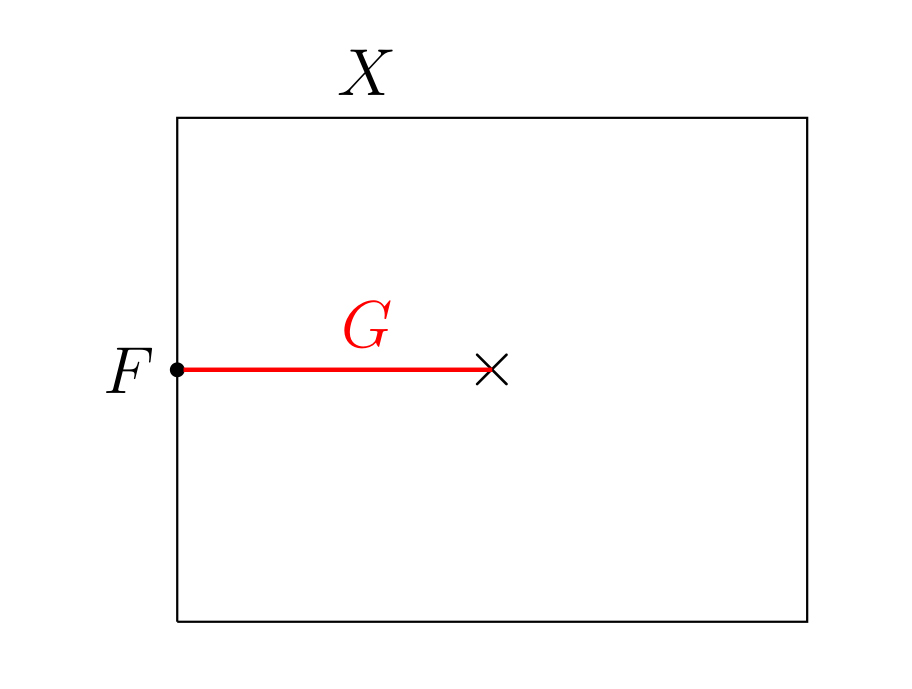
\includegraphics[width=0.40\textwidth]{figures/fig4_1.png}
\caption{相对停点。图内 $X$ 为流形，$F$ 与 $G$ 为相对停点的两个部分。}
\label{fig:rel-stop}
\end{figure}

\begin{thmstar}
设 $X$ 是光滑仿射簇，带嵌入 $X\to\C^N$，该嵌入在 $X$ 上诱导 Stein 结构；设
$f,g\colon X\to\C$ 是 $\C^N$ 上多项式函数的限制。若 $f$ 只有一个临界纤维
$f^{-1}(0)$，则对充分小的 $t\neq0$，存在全忠实函子
\[
\cW(f^{-1}(t),g)\to\cW(X\times\C,z(f-t),g).
\]
\end{thmstar}

\transnote{易错预警：原书在此重述引言中的定理 \ref{thm:relative}（相对版本），并沿用原编号。
译本同样用无编号的 thmstar 环境重述，编号引定理 \ref{thm:relative}，以免自动编号另起
新号、把后文的定义挤位。}

这里第二个范畴关于 $g$ 逐纤维带停点，如 [AA21] 中那样：可容拉格朗日子流形在原映射
$f\colon X\to\C$ 下纤维化于弧之上，同时在 $f$ 的纤维内关于限制 $g|_{f^{-1}(t)}$ 可容。

\begin{definition}\label{def:4-1-1}
给定 Stein 流形 $X$ 与两个全纯函数 $f,g\colon X\to\C$，定义相对 Fukaya--Seidel 范畴
（relative Fukaya--Seidel category）$\cW(X,f,g)$ 为 $X$ 的 wrapped Fukaya 范畴
$\cW(X,F\cup G)$，其相对停点（relative stop）由以下两者的并给出：
\begin{itemize}
\item $F$：扇形 $(f^{-1}(-\infty),g)$ 的相对骨架（relative skeleton），位于
$\partial^\infty X$ 内；
\item $G$：$(g|_{f^{-1}(t)})^{-1}(-\infty)\subseteq\partial^\infty f^{-1}(t)\subseteq
\partial^\infty X$ 的并，其中 $t$ 沿一条连接 $-\infty$ 与 $0$ 的弧取值；
\end{itemize}
如图 \ref{fig:rel-stop} 所示。
\end{definition}

\transnote{易错预警：定义 \ref{def:4-1-1} 中的 $F$、$G$ 是两族边界集，不是函数。相对
停点取 $F\cup G$：$F$ 是扇形 $(f^{-1}(-\infty),g)$ 的相对骨架，$G$ 是沿一条弧变化的一族
停点之并。后文说「附加手柄的余核 $\ell$」时，$\ell$ 与这里的 $F$、$G$ 无关。}

这个停点可以看作相对骨架在无穷远处的边界。

\transnote{含糊点拨：原书这句跨 p.64--65，且页图在 p.64 末行与 p.65 首行重复出现
「relative skeleton」，疑为底本笔误。译文合并为一句，只保留一次「相对骨架」，并在报告
疑点中列明。}
